\documentclass[border=8pt]{standalone}
\usepackage{xcolor}
\usepackage{tikz}
\usepackage{helvet}
\renewcommand{\familydefault}{\sfdefault}
\definecolor{epflred}{RGB}{255,0,0}
\definecolor{ink}{RGB}{24,24,24}
\definecolor{muted}{RGB}{102,102,102}
\begin{document}
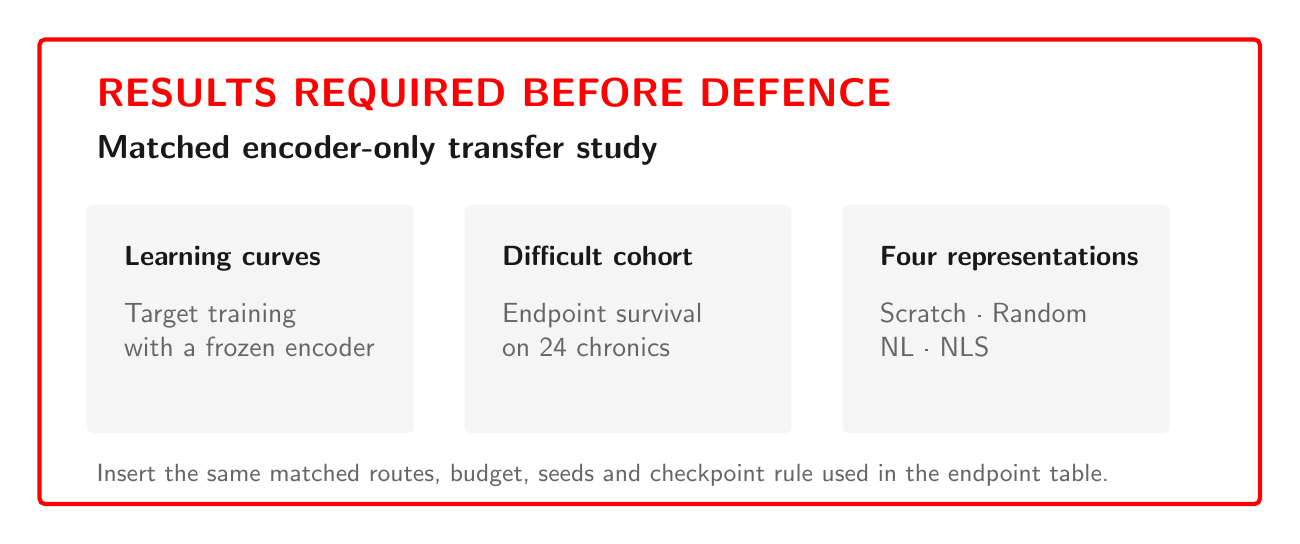
\begin{tikzpicture}
  \fill[white] (0,0) rectangle (15.8,6.2);
  \draw[epflred, line width=1.5pt, rounded corners=2pt] (0.15,0.15) rectangle (15.65,6.05);
  \node[anchor=west, text=epflred, font=\bfseries\Large] at (0.75,5.35) {RESULTS REQUIRED BEFORE DEFENCE};
  \node[anchor=west, text=ink, font=\bfseries\large] at (0.75,4.65) {Matched encoder-only transfer study};
  \fill[black!4, rounded corners=2pt] (0.75,1.05) rectangle +(4.15,2.9);
  \node[anchor=north west, text=ink, font=\bfseries\normalsize, align=left] at (1.10,3.55) {Learning curves};
  \node[anchor=north west, text=muted, font=\normalsize, align=left] at (1.10,2.82) {Target training\\with a frozen encoder};
  \fill[black!4, rounded corners=2pt] (5.55,1.05) rectangle +(4.15,2.9);
  \node[anchor=north west, text=ink, font=\bfseries\normalsize, align=left] at (5.90,3.55) {Difficult cohort};
  \node[anchor=north west, text=muted, font=\normalsize, align=left] at (5.90,2.82) {Endpoint survival\\on 24 chronics};
  \fill[black!4, rounded corners=2pt] (10.35,1.05) rectangle +(4.15,2.9);
  \node[anchor=north west, text=ink, font=\bfseries\normalsize, align=left] at (10.70,3.55) {Four representations};
  \node[anchor=north west, text=muted, font=\normalsize, align=left] at (10.70,2.82) {Scratch · Random\\NL · NLS};
  \node[anchor=west, text=muted, font=\small] at (0.75,0.52) {Insert the same matched routes, budget, seeds and checkpoint rule used in the endpoint table.};
\end{tikzpicture}
\end{document}
